\documentclass[12pt, a4paper]{article}
\usepackage[utf8]{inputenc}
\usepackage[english]{babel}
\usepackage[ruled]{algorithm2e}
\usepackage{aligned-overset}
\usepackage{alltt}
\usepackage{amssymb}
\usepackage{amsmath}
\usepackage{amsthm}
\usepackage{mathtools}
\usepackage{bbm}
\usepackage{csquotes}
\usepackage{enumerate}
\usepackage{multicol}
\usepackage{stmaryrd}
\usepackage{subcaption}
\usepackage{xcolor}
\usepackage{tikz}
\usepackage{graphicx}
\usepackage{float}

\DeclarePairedDelimiter\abs{\lvert}{\rvert}%
\DeclarePairedDelimiter\norm{\lVert}{\rVert}%

\DeclarePairedDelimiter\bra{\langle}{\rvert}
\DeclarePairedDelimiter\ket{\lvert}{\rangle}
\DeclarePairedDelimiterX\braket[2]{\langle}{\rangle}{#1 \delimsize\vert #2}
\newcommand{\braketmatrix}[3]{\left \langle #1 \middle| #2 \middle| #3 \right \rangle}
\newcommand{\observable}[1]{\langle #1 \rangle}
\newcommand{\statepsi}[0]{\ket{\psi}}

\newcommand\todo[1]{\textcolor{red}{\textbf{TODO: #1}}}

\newtheorem{thm}{Theorem}
\newtheorem{definition}[thm]{Definition}
\newtheorem{corollary}[thm]{Corollary}
\newtheorem{lemma}[thm]{Lemma}

\begin{document}
\title{Notes on Introduction to Quantum Computing}
\author{Leon Windheuser}

\maketitle

\section{Basic Concepts}
\subsection{Quantum bits (qubits)}

Classical bits: $0, 1$ \newline
Quantum bit \textit{qubit}: Superposition of $0$ and $1$:

A quantum state $\ket{\psi}$ is described as 
\begin{equation}
    \ket{\psi} := \alpha \ket{0} + \beta \ket{1}, \quad \alpha, \beta \in \mathbb{C} 
\end{equation}
where 
\begin{equation}
    \abs{\alpha}^2 + \abs{\beta}^2 = 1 \quad \text(normalization).
\end{equation}
%
Mathematical description: $\ket{\psi} \in \mathbb{C}^2$ with
\begin{equation*}
    \ket{0} = \begin{pmatrix}1 \\ 0 \end{pmatrix}, 
    \quad \ket{1} = \begin{pmatrix}0 \\ 1\end{pmatrix}
    \quad \leadsto \ket{\psi} = \begin{pmatrix}
        \alpha \\ \beta
    \end{pmatrix}
\end{equation*}


Different from classical bits, cannot (in general) directly observe / measure a qubit 
(the amplitudes $\alpha$ and $\beta$).
%
Instead: "\textit{standard}" measurement will result in 
\begin{itemize}
    \item $0$ with probability $\abs{\alpha}^2$
    \item $1$ with probability $\abs{\beta}^2$
\end{itemize}
%

The measurement also \underline{changes} the qubit (\textit{wavefunction collapse}).
%
If measuring $0$, the qubit will be $\ket{\psi} = \ket{0}$ directly after the measurement,
and likewise if measuring $1$, the qubit will be $\ket{\psi} = \ket{1}$. \newline

In practise: Can estimate the probabilities $\abs{\alpha}^2$ and $\abs{\beta}^2$ in 
experiments by repeating the same experiment many times (i.e via outcome statistics).
These repetitions are called \textit{trials} or \textit{shots}.

\begin{figure}[h]
    \centering
    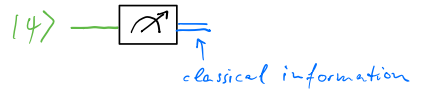
\includegraphics[scale=0.5]{chapters/res/circuit-notation.png}
    \caption{Circuit notation}
\end{figure}
\newpage

A useful graphical deputation of a qubit is the \underline{Bloch sphere} representation:
If $\alpha$ and $\beta$ happen to be real-valued, then can find angle 
$\vartheta \in \mathbb{R}$ such that
\begin{equation}
    \alpha = \cos{\frac{\vartheta}{2}}, \quad \beta = \sin{\frac{\vartheta}{2}}
\end{equation}
\begin{equation*}
    (\leadsto \abs{\alpha}^2 + \abs{\beta}^2 
    = \cos{\frac{\vartheta}{2}} + \sin{\frac{\vartheta}{2}}) = 1 \quad \color{green}\checkmark
\end{equation*}

\begin{figure}[h]
    \centering
    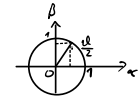
\includegraphics[scale=0.5]{chapters/res/bloch_sphere_sin_cos.png}
\end{figure}

In general: represent 
\begin{align*}
    \alpha &= e^{i \gamma} \cos{\frac{\vartheta}{2}} \\
    \beta &= e^{i (\varphi + \gamma)} \sin{\frac{\vartheta}{2}} \\
\end{align*}
using so-called phase angles $\gamma$ for $\alpha$ and $\varphi + \gamma$ for $\beta$.

\begin{figure}[h]
    \centering
    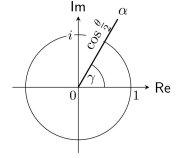
\includegraphics[scale=0.6]{chapters/res/sin-cos-complex.png}
\end{figure}

Then:
\begin{align}
    \ket{\psi} &= 
        e^{i \psi} \cos{\frac{\vartheta}{2}} \cdot \ket{0} 
        + \underbrace{e^{i (\varphi + \gamma)}}_{= \text{ } e^{i\varphi} \cdot e^{i\gamma}} \sin{\frac{\vartheta}{2}} \cdot \ket{1} \\
        %
        &= \underbrace{e^{i \gamma}}_{\text{can be ignored here}}
        \left(\cos{\frac{\vartheta}{2}} \cdot \ket{0} + e^{i\varphi} \cdot \sin{\frac{\vartheta}{2}} \cdot \ket{1}\right)
\end{align}

Thus $\ket{\psi}$ is characterized by two angles $\varphi$ and $\gamma$;
these specify the point defined as 
\begin{equation*}
    \vec{r} = \begin{pmatrix}
        \cos{\varphi} \cdot \sin{\vartheta} \\
        \sin{\varphi} \cdot \sin{\vartheta} \\
        \cos{\vartheta}
    \end{pmatrix}
\end{equation*}

on the surface of a sphere:
\begin{figure}[h!]
    \centering
    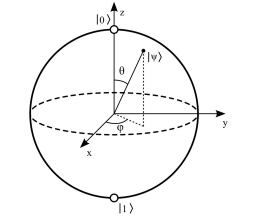
\includegraphics[scale=0.5]{chapters/res/bloch-sphere.png}
    \caption{Bloch Sphere (Felix Bloch)}
\end{figure}

\subsection{Single qubit gates}

Principles of \underline{time evolution}: The quantum state $\ket{\psi}$ at current
time point $t$ transitions to a new quantum state $\ket{\psi'}$ at a later time point
$t' > t$. \newline
Transition described by a complex unitary matrix $U$:
\begin{equation}
    \ket{\psi'} = U \cdot \ket{\psi}
\end{equation}

\begin{figure}[h!]
    \centering
    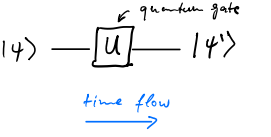
\includegraphics[scale=0.5]{chapters/res/circuit_time_evolution.png}
    \caption{Circuit notation}
\end{figure}

Notes: 
\begin{itemize}
    \item Circuit is read from left to right, but matrix times vector ($U\ket{\psi}$) from right to left.
    \item $U$ preserves normalization
\end{itemize}

Examples:
\begin{itemize}
    \item Quantum analogue of the classical NOT gate ($0 \leftrightarrow 1$) flip
    $\ket{0} \leftrightarrow \ket{1}$ leads to Pauli-X gate:
    \begin{equation}
        X \equiv \sigma_1 = \begin{pmatrix}
            0 & 1 \\
            1 & 0
        \end{pmatrix}
    \end{equation}

    Check: $X\ket{0} = \begin{pmatrix}
            0 & 1 \\
            1 & 0
        \end{pmatrix} \begin{pmatrix}0 \\ 1 \end{pmatrix} = \ket{1}$ and 
        $X\ket{1} = \begin{pmatrix}
            0 & 1 \\
            1 & 0
        \end{pmatrix} \begin{pmatrix}1 \\ 0 \end{pmatrix} = \ket{0} 
        \quad \color{green}\checkmark $
    
    \item Pauli-Y gate: 
    \begin{equation}
        Y \equiv \sigma_2 = \begin{pmatrix}
            0 & -i \\
            i & 0
        \end{pmatrix}
    \end{equation}

    \item Pauli-Z gate: 
    \begin{equation}
        Z \equiv \sigma_3 = \begin{pmatrix}
            1 & 0 \\
            0 & -1
        \end{pmatrix}
    \end{equation}

    Z leaves $\ket{0}$ unchanged, but flips the sign of the coefficient of $\ket{1}$.
    Recall the Bloch Sphere representation:
    \begin{equation*}
        \ket{\psi} = \cos{\frac{\vartheta}{2}} \cdot \ket{0} + e^{i\varphi} \sin{\frac{\vartheta}{2}} \cdot \ket{1}
    \end{equation*} 

    Then
    \begin{align*}
        Z \ket{\psi} &= \cos{\frac{\vartheta}{2}} \cdot \ket{0} {\color{red}\text{ }-\text{ }}
            e^{i\varphi} \sin{\frac{\vartheta}{2}} \cdot \ket{1} \\
        %
        &\stackrel{e^{i\pi} = -1}{=} \cos{\frac{\vartheta}{2}} \cdot \ket{0} + 
            \underbrace{e^{i\pi} e^{i\varphi}}_{e^{i(\varphi + \pi)}} \sin{\frac{\vartheta}{2}} \cdot \ket{1}
    \end{align*}

    $\leadsto$ new Bloch Sphere angles: $\vartheta' = \vartheta, \varphi = \varphi + \pi$ 
    (rotating by $\pi = 180^\circ$ around z-axis) \newline
    X, Y, Z gates are called \underline{Pauli matrices}.
    The \underline{Pauli vector} $\vec{\sigma} = (\sigma_1, \sigma_2, \sigma_3) = (X, Y, Z)$
    is a vector of $2 \times 2$ matrices.

    \item Hadamard Gate:
    \begin{equation*}
        H = \frac{1}{\sqrt{2}}  \begin{pmatrix}
            1 & 1 \\
            1 & -1
        \end{pmatrix}
    \end{equation*}

    \begin{figure}[h]
        \centering
        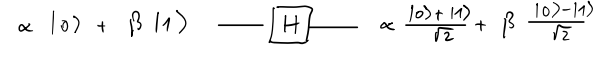
\includegraphics[scale=0.5]{chapters/res/hadamard-gate-circuit.png}
        \caption{Hadamard Gate}
    \end{figure}

    \item Phase Gate:
    \begin{equation*}
        S = \begin{pmatrix}
            1 & 0 \\
            0 & i
        \end{pmatrix}
    \end{equation*}

    \item T Gate:
    \begin{equation*}
        T = \begin{pmatrix}
            1 & 0 \\
            0 & e^{i\pi/4}
        \end{pmatrix}
    \end{equation*}
    Note: $T^2 = S$ since $(e^{i \pi /4})^2 = e^{i\pi/2} = i$
\end{itemize}


Pauli matrices satisfy:
\begin{enumerate}
    \item $\sigma^{2}_{j} = I$ (identifity) for $j = 1,2,3$
    \item $\sigma_j \cdot \sigma_k = - \sigma_k \sigma_j$ for all $j \neq k$
    \item ${\color{blue} [} \sigma_j, \sigma_k {\color{blue} ]} :=
        \underbrace{\sigma_j \sigma_k - \sigma_k \sigma_j}_{\text{Commutator}} = 
        2 i \sigma_l$ for $(j,k,l)$ a cyclic permutation of (1,2,3).
\end{enumerate}

General definition of \underline{matrix exponential}

\begin{equation}
    exp(A) \equiv e^A = \sum_{k = 0}^{\infty} \frac{1}{k!}A^k, \quad A \in \mathbb{C}^{n \times n}
\end{equation}

Special case: $A^2 = I, x \in \mathbb{R}$
\begin{align*}
    e^{i A x} &= \underbrace{\sum_{k = 0}^{\infty} \frac{1}{(2k)!} (ix)^{2k} 
        \underbrace{A^{2k}}_{(A^2)^k = I^k = I}}_\text{even} +
        \underbrace{\sum_{k = 0}^{\infty} \frac{1}{(2k + 1)!} (ix)^{2k + 1} 
            \underbrace{A^{2k+1}}_{(A^2)^k \cdot A = I^k \cdot A= A}}_\text{odd} \\
        &= \underbrace{\sum_{k = 0}^{\infty} \frac{1}{(2k)!} (-1)^k x^{2k}}_{ = \cos{x}} \cdot I +
        \underbrace{\sum_{k = 0}^{\infty} \frac{1}{(2k + 1)!} (-1)^k x^{2k + 1}}_{=i \sin{x}} \cdot A\\
        &= \cos{x} \cdot I + i \sin{x} A
\end{align*}
(generalizes Euler's formula $e^{ix} = \cos{x} + i \sin{x}$)
\newline

This can be used to define the following \underline{rotation operators} via the
Pali matrices. Let $\vartheta \in \mathbb{R}$:

\begin{align}
    R_x(\vartheta) &:= e^{-i \vartheta X / 2} 
        = \cos{\frac{\vartheta}{2}} I - i \sin{\frac{\vartheta}{2}} X 
        = \begin{pmatrix}
            \cos{\frac{\vartheta}{2}} & -i \sin{\frac{\vartheta}{2}} \\
            -i \sin{\frac{\vartheta}{2}} & \cos{\frac{\vartheta}{2}}
        \end{pmatrix} \\
    %
    R_y(\vartheta) &:= e^{-i \vartheta Y / 2} 
        = \cos{\frac{\vartheta}{2}} I - i \sin{\frac{\vartheta}{2}} Y 
        = \begin{pmatrix}
            \cos{\frac{\vartheta}{2}} & -\sin{\frac{\vartheta}{2}} \\
            \sin{\frac{\vartheta}{2}} & \cos{\frac{\vartheta}{2}}
        \end{pmatrix} \\ 
    R_z(\vartheta) &:= e^{-i \vartheta Z / 2} 
        = \cos{\frac{\vartheta}{2}} I - i \sin{\frac{\vartheta}{2}} Z
        = \begin{pmatrix}
            e^{-i \vartheta / 2} & 0 \\
            0 & e^{i \vartheta / 2}
        \end{pmatrix}
\end{align} 
\newpage


General case: Rotation about an axis $\vec{v} \in \mathbb{R}^3$
(normalized such that $\norm{\vec{v}}) = \sqrt{v_1^2 + v_2^2 + v_3^3} = 1$): \newline
using the notation:

\begin{equation}
    \braket{\vec{v}}{\vec{\sigma}} 
        = \vec{v} \cdot \vec{\sigma} 
        = v_1 \sigma_1 + v_2 \sigma_2 + v_3 \sigma_3
        = \begin{pmatrix}
            v_3 && v_1 - i v_2 \\
            v_1 + i v_2 && -v_3
        \end{pmatrix}
\end{equation}

It holds that $(\vec{v} \cdot \vec{\sigma})^2 = I$.

We define the rotation operator around axis $\vec{v}$ as 
\begin{equation}
    R_v(\vartheta) := e^{-i \vartheta (\vec{v} \cdot \vec{\sigma}) / 2} 
        = \cos{\frac{\vartheta}{2}} I - i \sin{\frac{\vartheta}{2}} (\vec{v} \cdot \vec{\sigma})
\end{equation}

Note: $R_x$, $R_y$, $R_z$ are special cases corresponding to $\vec{v} = (1, 0, 0)$, 
$\vec{v} = (0, 1, 0)$, and $\vec{v} = (0, 0, 1)$. \newline 

Can derive that the Bloch Sphere representaiton of $R_{\vec{v}}(\vartheta)$ 
is a "conventional" rotation (in three dimensions) by angle $\vartheta$ about 
axis $\vec{v}$.

\begin{figure}[h]
    \centering
    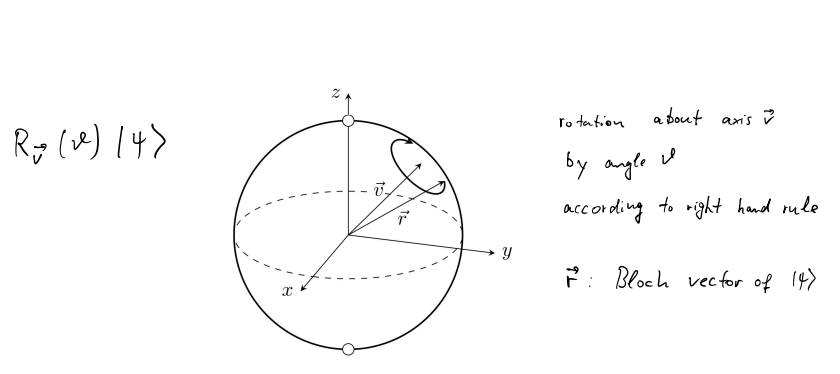
\includegraphics[scale=0.5]{chapters/res/bloch-sphere-rotation.png}
    \caption{Circuit notation}
\end{figure}


\underline{Z-Y decomposition} of an arbitrary $2 \times 2$ unitary matrix: \newline
For any unitary matrix $U \in \mathbb{C}^{n \times n}$ there exist real numbers
$\alpha, \beta, \gamma, \delta \in \mathbb{R}$ such that

\begin{equation}
    U = e^{i \alpha} \underbrace{\begin{pmatrix}
        e^{-i \beta / 2} & 0 \\
        0 & e^{i \beta / 2} 
    \end{pmatrix}}_{R_z(\beta)} \cdot 
    \underbrace{\begin{pmatrix}
        \cos{\frac{\gamma}{2}} & -\sin{\frac{\gamma}{2}} \\
        \sin{\frac{\gamma}{2}} & \cos{\frac{\gamma}{2}}
    \end{pmatrix}}_{R_y(\gamma)} \cdot 
    \underbrace{\begin{pmatrix}
        e^{-i \delta / 2} & 0 \\
        0 & e^{i \delta / 2} 
    \end{pmatrix}}_{R_z(\delta)}
\end{equation}

\subsection{Multiple qubits}

So far: Single qubits, superposition of basis states $\ket{0}$ and $\ket{1}$.
For two qubits, this generalizes to $\{\ket{00}, \ket{01}, \ket{10}, \ket{11}\}$. \newline

General two-qubit state:
\begin{equation}
    \ket{\psi} = \alpha_{00} \ket{00} + \alpha_{01} \ket{01} + \alpha_{10} \ket{10} + \alpha_{11} \ket{11}
\end{equation}
with amplitudes $\alpha_{ij} \in \mathbb{C}$ such that
\begin{equation}
    \abs{\alpha_{00}}^2  + \abs{\alpha_{01}}^2  + \abs{\alpha_{10}}^2  + \abs{\alpha_{11}}^2 = 1 
    \quad \text{(normalization).}
\end{equation}

Can identify the basis states with unit vectors:

\begin{equation}
    \ket{00} = \begin{pmatrix*}
        1 \\ 0 \\ 0 \\ 0
    \end{pmatrix*} \quad
    \ket{01} = \begin{pmatrix*}
        0 \\ 1 \\ 0 \\ 0
    \end{pmatrix*} \quad
    \ket{10} = \begin{pmatrix*}
        0 \\ 0 \\ 1 \\ 0
    \end{pmatrix*} \quad
    \ket{11} = \begin{pmatrix*}
        0 \\ 0 \\ 0 \\ 1
    \end{pmatrix*} \quad
\end{equation}

Thus: 
\begin{equation}
    \ket{\psi} = \begin{pmatrix*}
        \alpha_{00} \\ \alpha_{01} \\ \alpha_{10} \\ \alpha_{11} 
    \end{pmatrix*} \in \mathbb{C}^4
\end{equation}

What happens if we measure only one qubit of a two-qubit state?
Say we measure the first qubit: Obtain result
\begin{align*}
    0 &\quad \text{with probability} \quad \abs{\alpha_{00}}^2 + \abs{\alpha_{01}}^2 \\ 
    1 &\quad \text{with probability} \quad \abs{\alpha_{10}}^2 + \abs{\alpha_{11}}^2
\end{align*}

Wavefunction directly after measurement:
\begin{align*}
    &\text{if measured 0:} \quad \ket{\psi'} 
        = \frac{\alpha_{00}\ket{00} + \alpha_{01}\ket{01}}{\sqrt{\abs{\alpha_{00}}^2 + \abs{\alpha_{01}}^2}} \\
    &\text{if measured 1:} \quad \ket{\psi'} 
        = \frac{\alpha_{10}\ket{10} + \alpha_{11}\ket{11}}{\sqrt{\abs{\alpha_{10}}^2 + \abs{\alpha_{11}}^2}} \\
\end{align*}


Mathematical formalism for constructing two qubit states: Tensor product of vector space. \newline
Can combine two (arbitrary) vector spaces $V$ and $W$ to form the \underline{tensor product}
$V \otimes W$. \\
The elements of $V \otimes W$ are linear combinations of "tensor products" 
$\ket{v} {\color{blue} \otimes} \ket{w}$ consisting of elements $\ket{v} \in V$ and  $\ket{w} \in W$. \\

Example: Let $V = \mathbb{C}^2$ and $W = \mathbb{C}^2$ be the single qubit spaces with basis
$\{\ket{0}, \ket{1}\}$, then

\begin{equation*}
    \underbrace{\frac{1}{2} \ket{0} {\color{blue} \otimes} \ket{0}}_{=\ket{00}} + 
    \underbrace{\frac{5i}{7} \ket{1} {\color{blue} \otimes} \ket{0}}_{=\ket{10}} 
    \in V \otimes W
\end{equation*}

Let $\{\ket{i}_v : i = 1, ... ,m\}$ be a basis of of V, and 
let $\{\ket{j}_w : j = 1, ... ,n\}$ be a basis of of W, then

\begin{equation*}
    \{\ket{i}_v {\color{blue}\otimes} \ket{j}_w : i = 1,...,m, j = 1,...,n \}    
\end{equation*}
is a basis of $V {\color{blue} \otimes} W$.
In particular, $dim(V \otimes W) = dim(V) \cdot dim(W)$.\\ 
Note: $\ket{i}_v {\color{blue}\otimes} \ket{j}_w$ is also written as $\ket{ij}$. \\

Basic properties of tensor product:
\begin{itemize}
    \item $\forall \ket{v} \in V, \ket{w} \in W \land \alpha \in \mathbb{C}:$
    \begin{equation}
        \alpha (\ket{v} \otimes \ket{w}) 
            = (\alpha \ket{0}) \otimes \ket{w} 
            = \ket{v} \otimes (\alpha \ket{w})
    \end{equation}

    \item $\forall \ket{v_1}, \ket{v_2} \in V \land \ket{w} \in W:$
    \begin{equation}
        (\ket{v_1} + \ket{v_2}) \otimes \ket{w} 
            = \ket{v_1} \otimes \ket{w} + \ket{v_2} \otimes \ket{w}
    \end{equation}

    \item $\forall \ket{v} \in V \land \ket{w_1}, \ket{w_2} \in W:$
    \begin{equation}
        \ket{v} \otimes (\ket{w_1} + \ket{w_2})
            = \ket{v} \otimes \ket{w_1} + \ket{v} \otimes \ket{w_2}
    \end{equation}
\end{itemize}

Vector notation using standard basis, e.g.
\begin{align*}
    \ket{v} &= v_1\ket{0} + v_2\ket{1} = \begin{pmatrix*}
        v_1 \\ v_2
    \end{pmatrix*} \\
    \ket{w} &= w_1\ket{0} + w_2\ket{1} = \begin{pmatrix*}
        w_1 \\ w_2
    \end{pmatrix*} \\
    \ket{v} \otimes \ket{w} &= (v_1\ket{0} + v_2\ket{1}) \otimes (w_1\ket{0} + w_2\ket{1}) \\
    &= v_1 w_1 \ket{00} + v_1 w_2 \ket{01} + v_2 w_1 \ket{10} + v_2 w_2 \ket{11}
\end{align*}

Thus: 
\begin{equation*}
    \begin{pmatrix*}
        v_1 \\ v_2
    \end{pmatrix*} \otimes
    \begin{pmatrix*}
        w_1 \\ w_2
    \end{pmatrix*} = 
    \begin{pmatrix*}
        v_1 w_1 \\ v_1 w_2 \\ v_2 w_1 \\ v_2 w_2
    \end{pmatrix*}
\end{equation*}


Note: Not every element of $V \otimes W$ can be written in the form $\ket{v} \otimes \ket{w}$,
for example the Bell state
\begin{equation*}
    \ket{\psi} = \frac{1}{\sqrt{2}} (\ket{00} + \ket{11}).
\end{equation*}

Assuming that $V$ and $W$ have an inner product $\braket{\cdot}{\cdot}$, define inner product
on $V \otimes W$ by

\begin{equation}
    \braket{\sum_j \alpha_j \ket{v_j} \otimes \ket{w_j}}
        {\sum_k \beta_k \ket{v_k} \otimes \ket{w_k}} :=
    \sum_j \sum_k \alpha_j^* \beta_k \braket{v_j}{v_k}\cdot \braket{w_j}{w_k}
\end{equation}


Generalization to $n$ qubits: $2^n$ computational basis states
\begin{equation*}
    \{\underbrace{\ket{0, ..., 0}}_{\text{length $n$}}, \ket{0, ..., 0, 1}, ... \ket{1,...,1}\}
\end{equation*}

Thus: General n-qubit quantum state, also denoted as "quantum register", given by:

\begin{equation}
    \ket{\psi} = \sum_{x_0 = 0}^1 \sum_{x_1 = 0}^2 \cdots \sum_{x_{n-1}}^1 \alpha_{x_n-1,..., x_1, x_0}
        \cdot \ket{x_{n-1},..., x_1 x_0}
\end{equation}

with $\alpha_x \in \mathbb{C}$ for all $x \in \{0, ..., 2^n - 1\}$, such that 
$\norm{\psi}^2 = \sum_{x = 0}^{2^n - 1} \abs{\alpha_x}^2 = 1$ (normalization).

$\leadsto$ In general \textit{"hard"} to simulate on classical computer (for large $n$) due to "curse of dimensionality". \\
Vector space as tensor products: 
$\underbrace{\mathbb{C}^2 \otimes \cdots \otimes \mathbb{C}^2}_{\text{$n$ times}} 
= (\mathbb{C}^2)^{\otimes n} = \mathbb{C}^{(2^n)}$

\subsection{Multiple qubit gates}

As for single qubits, an operation on multiple qubits is described by an unitary matrix $U$.
For $n$ qubits: $U \in \mathbb{C}^{2^n \times 2^n}$
\newpage
%
Example: \underline{controlled-NOT} gate (also CNOT): \\
two qubits: {\color{orange}control} and target, target qubit gets flipped if {\color{orange}control} is 1: \\

\begin{equation*}
    \ket{{\color{orange}0}0} \mapsto \ket{00}, 
    \quad \ket{{\color{orange}0}1} \mapsto \ket{01}, 
    \quad \ket{{\color{orange}1}0} \mapsto \ket{11}, 
    \quad \ket{{\color{orange}1}1} \mapsto \ket{11}
\end{equation*}

Can be expressed as
\begin{equation}
    \ket{a, b} \mapsto \ket{a, a \oplus b} \quad \forall a, b \in \{0, 1\}
\end{equation}
, where $\oplus$ is the addition modulo 2.

\begin{figure}[h]
    \centering
    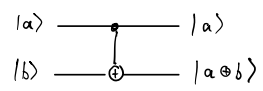
\includegraphics[scale=0.5]{chapters/res/cnot-circuit.png}
    \caption{CNOT circuit notation}
\end{figure}

Matrix representation:

\begin{equation}
    U_{CNOT} = \begin{pmatrix*}
        1 && 0 && 0 && 0 \\
        0 && 1 && 0 && 0 \\
        0 && 0 && \color{red} 0 && \color{red} 1 \\
        0 && 0 && \color{red} 1 && \color{red} 0 \\
    \end{pmatrix*}
\end{equation},
with the Pauli-X matrix $X = \begin{pmatrix*}
        \color{red} 0 && \color{red} 1 \\
        \color{red} 1 && \color{red} 0 \\
\end{pmatrix*}$.
 
\begin{figure}[h]
    \centering
    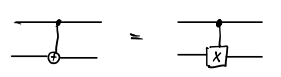
\includegraphics[scale=0.5]{chapters/res/cnot-alternative-circuit.png}
    \caption{Alternative CNOT circuit notation}
\end{figure}

Can generalize Pauli-X to any unitary operator U acting on target qubit $\leadsto$ 
\textbf{controlled-U gate}:

\begin{equation*}
    \ket{{\color{orange}0}0} \mapsto \ket{00}, 
    \quad \ket{{\color{orange}0}1} \mapsto \ket{01}, 
    \quad \ket{{\color{orange}1}0} \mapsto \ket{1} {\color{blue} \otimes} (U\ket{0}), 
    \quad \ket{{\color{orange}1}1} \mapsto \ket{1} {\color{blue} \otimes} (U\ket{1})
\end{equation*}

\begin{figure}[H]
    \centering
    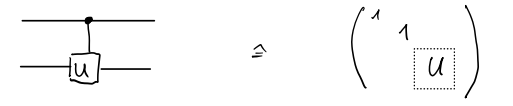
\includegraphics[scale=0.5]{chapters/res/contolled-u-gate-circuit.png}
    \caption{Controlled-U gate}
\end{figure}

\begin{figure}[H]
    \centering
    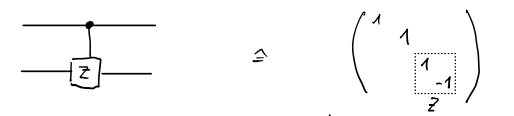
\includegraphics[scale=0.5]{chapters/res/controlled-z-gate-circuit.png}
    \caption{Example: Controlled-Z gate}
\end{figure}

\begin{figure}[H]
    \centering
    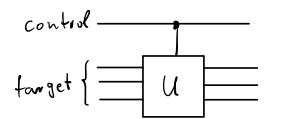
\includegraphics[scale=0.5]{chapters/res/controlled-u-multiple-targets.png}
    \caption{Controlled-U for multiple target qubits}
\end{figure}

Note: Single qubit and CNOT gates are \underline{universal}: They can be used to implement an 
arbitraty unitray operation on $n$ qubits (Quantum analogue of univerisity of classical NAND gate).
Proof in Nielsen and Chuang section 4.5.

\begin{figure}[H]
    \centering
    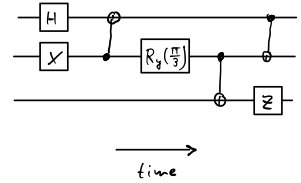
\includegraphics[scale=0.5]{chapters/res/example-qubit-single-qubit-gates-cnot.png}
    \caption{Example of a circuit lousisting only of single qubit gates and CNOTs}
\end{figure}

\subsubsection{Matrix Kronecker Products}
Matrix representation of single qubit gates acting in parallel:

\begin{figure}[H]
    \centering
    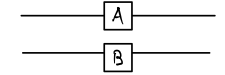
\includegraphics[scale=0.5]{chapters/res/parallel-circuit.png}
\end{figure}

Operation on basis states: $a, b \in \{0, 1\}$:
\begin{equation}
    \ket{a, b} \mapsto (A\ket{a}) \otimes (B\ket{b})
\end{equation}

Example: $A = I$ (identity), $B = Y$
\begin{align*}
    \ket{00} &\mapsto \ket{0} \otimes (Y\ket{0}) = {\color{purple}i}\ket{01} \\
    \ket{01} &\mapsto \ket{0} \otimes (Y\ket{1}) = {\color{green}-i} \ket{00} \\
    \ket{10} &\mapsto \ket{1} \otimes (Y\ket{0}) = i \ket{11} \\
    \ket{11} &\mapsto \ket{1} \otimes (Y\ket{1}) = -i \ket{10}
\end{align*}

Matrix representation:
\begin{equation*}
    \begin{pmatrix*}
        0 && \color{green} -i && 0 && 0 \\
        \color{purple} i && 0 && 0 && 0 \\
        0 && 0 && 0 && -i \\
        0 && 0 && i && 0 \\
    \end{pmatrix*} =
    \begin{pmatrix*}
        Y && 0 \\
        0 && Y
    \end{pmatrix*} = 
    I \otimes Y
\end{equation*}

\begin{figure}[H]
    \centering
    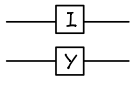
\includegraphics[scale=0.5]{chapters/res/parallel-circuit-i-y.png}
    \caption{Circuit notation}
\end{figure}

General formula: \underline{Kronecker product} (matrix representation of tensor products of operators)

\begin{equation}
    A \otimes B = \begin{pmatrix*}
        a_{11} B && a_{12} B && \cdots && a_{1n} B \\
        a_{21} B && a_{22} B && \cdots && a_{2n} B \\
        \vdots && \vdots && \ddots && \vdots \\
        a_{m1} B && a_{m2} B && \cdots && a_{mn} B \\
    \end{pmatrix*} \in
    \mathbb{C}^{mp \times nq} 
\end{equation}

for all $ A \in \mathbb{C}^{m \times n}$ and $B \in \mathbb{C}^{p \times q}$.

\begin{figure}[H]
    \centering
    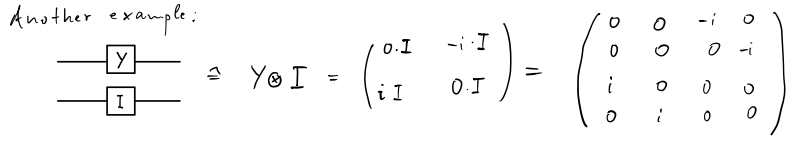
\includegraphics[scale=0.48]{chapters/res/kronecker-another-example.png}
\end{figure}

\begin{figure}[H]
    \centering
    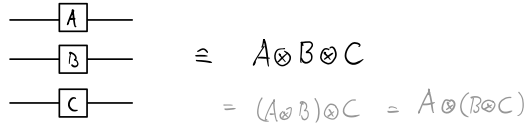
\includegraphics[scale=0.5]{chapters/res/kronecker-generlization-3-tensors.png}
    \caption{Generalization to arbitrary number of tensor factors possible}
\end{figure}

Basic properties:
\begin{enumerate}
    \item $(A \otimes B)^* = A^* \otimes B^*$ (elementwise complex conjugation)
    \item $(A \otimes B)^T = A^T \otimes B^T$ (transposition)
    \item $(A \otimes B)^\dag = A^\dag \otimes B^\dag$
    \item $(A \otimes B) \otimes C = A \otimes (B \otimes C)$ (associative property)
    \item $(A \otimes B) \cdot (C \otimes D) 
        = (A \cdot C) \otimes (B \cdot D)$ (for matrix of compatible dimensions)
        \begin{figure}[H]
            \centering
            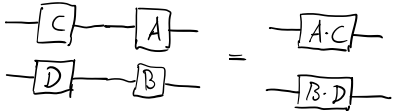
\includegraphics[scale=0.5]{chapters/res/kronecker-properties.png}
        \end{figure}
    \item Kronecker product of Hermitian matrices is Hermitian.
    \item Kronecker product of unitary matrices is unitary (follows from 3. and 5.)
\end{enumerate}

\subsection{Quantum measurement}
Review: measurement of a single qubit $\ket{\psi} = \alpha\ket{0} + \beta{\ket{1}}$ with
resepct to the computational basis $\{\ket{0}, \ket{1}\}$.

\begin{figure}[H]
    \centering
    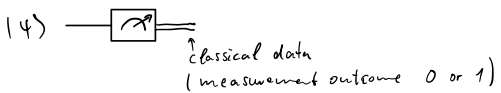
\includegraphics[scale=0.5]{chapters/res/quantum-measurement.png}
\end{figure}

Linear algebra: Can switch to a different (orthonormal) basis to represent a qubit, e.g.
\begin{align*}
    \ket{+} &= \frac{\ket{0} + \ket{1}}{\sqrt{2}} = \frac{1}{\sqrt{2}} \begin{pmatrix*}1 \\ 1\end{pmatrix*} \\
    \ket{-} &= \frac{\ket{0} - \ket{1}}{\sqrt{2}} = \frac{1}{\sqrt{2}} \begin{pmatrix*}1 \\ -1\end{pmatrix*}
\end{align*}

Representation of $\ket{\psi}$ w.r.t $\{\ket{+}, \ket{-}\}$ basis:
\begin{equation*}
    \alpha \ket{0} + \beta \ket{1} 
        = \alpha \frac{\ket{+} + \ket{-}}{\sqrt{2}} + \beta \frac{\ket{+} - \ket{-}}{\sqrt{2}}
        = \frac{\alpha + \beta}{\sqrt{2}} \ket{+} + \frac{\alpha - \beta}{\sqrt{2}} \ket{-}
\end{equation*}

Can perform measurement with resepct to orthonormal basis $\{\ket{+}, \ket{-}\}$, will obtain result
\begin{align*}
    + \quad &\text{with probability} \quad \frac{\abs{\alpha + \beta}^2}{2} \\
    - \quad &\text{with probability} \quad \frac{\abs{\alpha - \beta}^2}{2}
\end{align*}

Wavefunction collapse: immediately after the measurement, qubit will be in the state $\ket{+}$ if 
measured "+", likewise in the state $\ket{-}$ if measured "-".

\begin{figure}[H]
    \centering
    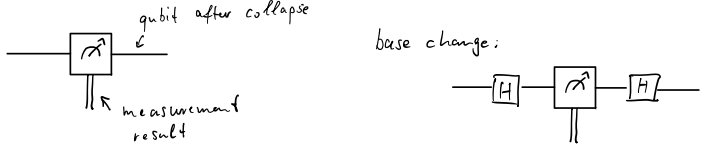
\includegraphics[scale=0.5]{chapters/res/measurement-collapse-basis.png}
\end{figure}

In general given an orthonormal basis $\{\ket{u_1}, \ket{u_2}\}$,
one can represent a qubit as $\ket{\psi} = \alpha_1 \ket{u_1} + \alpha_2 \ket{u_1}$
and measure with respect to this orthonormal basis;
will obtain measurement result $u_1$ or $u_2$ with respective probabilities $\abs{\alpha_1}^2$
and $\abs{\alpha_2}^2$.

\subsubsection{Abstract general definition of quantum measurements}
Quantum measurements are described by a collection $\{M_m\}$ of 
\underline{measurement} \underline{operators} acting on the quantum system, with the index $m$ labelling possible 
measurement outcomes. \\
Denoting the quantum state before measurement $\ket{\psi}$, result $m$ occurs with probability
\begin{equation}
    p(m) = \braketmatrix{\psi}{M_m^\dag M_m}{\psi} = \norm{M_m \ket{\psi}}^2
\end{equation}
, state after measurement is:
\begin{equation}
    \frac{M_m \ket{\psi}}{\norm{M_m \ket{\psi}}}
\end{equation}

The measurement operators satisfy the completeness relation

\begin{equation}
    \sum_m M_m^\dag M_m = I
\end{equation}

such that probabilities sum to 1:

\begin{equation}
    \sum_m p(m) 
        = \sum_m \braketmatrix{\psi}{M_m^\dag M_m}{\psi} 
        = \braketmatrix{\psi}{\sum_m M_m^\dag M_m}{\psi} \braket{\psi}{\psi} 
        = 1
\end{equation}
since $\sum_m M_m^\dag M_m = I$. \\
\newline
%
Example: measurement of a qubit $\ket{\psi} = \alpha \ket{0} + \beta \ket{1}$
with respect to computational basis $\{\ket{0}, \ket{\psi}\}$.

\begin{align*}
    M_0 &:= \ket{0} \bra{0} = \begin{pmatrix*}1 \\ 0\end{pmatrix*} (1, 0) = \begin{pmatrix*}
        1 && 0 \\ 0 && 0
    \end{pmatrix*} \\
    %
    M_1 &:= \ket{1} \bra{1} = \begin{pmatrix*}0 \\ 1\end{pmatrix*} (0, 1) = \begin{pmatrix*}
        0 && 0 \\ 0 && 1
    \end{pmatrix*} \\
    \leadsto p(0) &= \braketmatrix{\psi}{M_0^\dag M_0}{\psi} = \braketmatrix{\psi}{M_0}{\psi} = \abs{\alpha}^2 \\
    p(1) &= \braketmatrix{\psi}{M_1^\dag M_1}{\psi} = \braketmatrix{\psi}{M_1}{\psi} = \abs{\beta}^2 \\
\end{align*}

\subsubsection{Projective Measurements}
Projector onto subspace $V$ with orthonormal basis $\{\ket{u_1}, ..., \ket{u_m}\}$:
\begin{align}
    P &= \sum_{j = 1}^m \ket{u_j} \bra{u_j} \\
    P \ket{w} &= \sum_{j = 1}^m \underbrace{\braket{u_j}{w}}_{\text{inner product}}
\end{align}

Relation to spectral decomposition of a normal matrix $A \in \mathbb{C}^{n \times n}$:

\begin{align}
    A &= U \begin{pmatrix*}
        \lambda_1 & & \\
        & \ddots & \\
        & & \lambda_n
    \end{pmatrix*} U^\dag
    = \sum_{j = 1}^n \lambda_j \ket{u_j} \bra{u_j} \\
    &= \sum_{k = 1}^m \widetilde{\lambda_k} P_k \quad 
    \text{with } \{\widetilde{\lambda_1} ... \widetilde{\lambda_m} \} \text{ the distinct eigenvalues}
\end{align}

Definition:
A \underline{projective measurement} is described by an \underline{observable} $M$, 
a Hermitian operator acting on the quantum system.
Spectal decomposition:

\begin{equation}
    M = \sum_m \lambda_m P_m
\end{equation}

with $P_m$: projection onto eigenspace with eigenvalue $\lambda_m$.
The possible outcomes of the measurement correspond to the eigenvalues $\lambda_m$. \\
Probability of getting result $\lambda_m$ when measuring a quantum state $\ket{\psi}$:
\begin{equation}
    p(\lambda_m) = \braketmatrix{\psi}{P_m}{\psi}
\end{equation}

State of the quantum system directly after the measurement:

\begin{equation}
    \frac{P_m \ket{\psi}}{\norm{P_m \ket{\psi}}} = \frac{P_m \ket{\psi}}{\sqrt{p(\lambda_m)}}
\end{equation}

Remarks:
\begin{itemize}
    \item Projective measurements are special cases of general measurement framework
    \item Projective measurements combined with unitary transformations are equivalent to general
    measurement framework, see pages 94, 95 in Nielsen and Chuang.
\end{itemize}

Average value of a projective measurement:
\begin{align}
    \mathbb{E}[M] &= \sum_m \lambda_m p(\lambda_m) = \sum_m \lambda_m \braketmatrix{\psi}{P_m}{\psi} \\
    &= \braketmatrix{\psi}{\sum_m \lambda_m P_m}{\psi} = \braketmatrix{\psi}{M}{\psi} = \langle M \rangle
\end{align}

Corresponding \underline{standard deviation}:
\begin{equation}
   \Delta(M) := \sqrt{\langle M^2 \rangle - \langle M \rangle^2} 
        = \sqrt{\langle (M - \langle M \rangle)^2 \rangle}
\end{equation}

Examples:
\begin{itemize}
    \item Measuring a qubit w.r.t computational basis $\{ \ket{0}, \ket{1} \}$ is actually a projective measurement.
    \item In general: Measurement w.r.t orthonormal basis $\{\ket{u_1}, \ket{u_2}\}$ is a projective measurement: Set 
        \begin{equation*}
            P_m = \ket{u_m} \bra{u_m} \quad \text{for } m = 1, 2 
        \end{equation*}
        Define observable $M$ by 
        \begin{equation*}
            M := \sum_{m=1}^2 \lambda_m P_m \quad \text{with arbitrary } 
                \lambda_1, \lambda_2 \in \mathbb{R}; \lambda_1 \neq \lambda_2
        \end{equation*}
    \item Measuring Pauli-Z
    \begin{equation*}
        Z =  1 \cdot \underbrace{\begin{pmatrix*}
            1 && 0 \\
            0 && 0
        \end{pmatrix*}}_{P_1} + (-1) \cdot \underbrace{\begin{pmatrix*}
            0 && 0 \\
            0 && 1
        \end{pmatrix*}}_{P_2}
    \end{equation*}
    agrees with standard measurement w.r.t computational basis $\{ \ket{0}, \ket{1} \}$
\end{itemize}


\subsection{The Heisenberg uncertainty principle}

Suppose $A$ and $B$ are Hermitian operators, and $\ket{\psi}$ a quantum state.
Write 
\begin{equation}
    \braketmatrix{\psi}{AB}{\psi} = x + iy, \quad x, y \in \mathbb{R}
\end{equation}

\begin{equation}
     \braketmatrix{\psi}{AB}{\psi}^* 
        = \braketmatrix{\psi}{(AB)^\dag}{\psi} 
        = \braketmatrix{\psi}{B^\dag A^\dag}{\psi}
        = \braketmatrix{\psi}{BA}{\psi}
\end{equation}

Thus

\begin{equation}
    \braketmatrix{\psi}{[A, B]}{\psi} = 2iy \quad \text{and} \quad  \braketmatrix{\psi}{\{A, B \}}{\psi} = 2x
\end{equation}

where $\{A, B \} := AB + BA$ is the \underline{anti-Commutator}.

\begin{equation}\label{eq:star}
    \abs{\braketmatrix{\psi}{[A, B]}{\psi}}^2 +  \abs{\braketmatrix{\psi}{\{A, B\}}{\psi}}^2
        = 4  \cdot \underbrace{\abs{\braketmatrix{\psi}{AB}{\psi}}^2}_{x^2 + y^2}
\end{equation}

Cauchy-Schwarz inequality applied to $\ket{v} = A \ket{\psi}, \ket{w} = B \ket{\psi}$:

\begin{equation}
    \abs{\braketmatrix{\psi}{[A, B]}{\psi}}^2 
        \stackrel{\eqref{eq:star}}{\leq} 4 \cdot \abs{\braketmatrix{\psi}{AB}{\psi}}^2 
        \leq  4 \cdot \braketmatrix{\psi}{A^2}{\psi} \cdot \braketmatrix{\psi}{B^2}{\psi}
\end{equation}

Suppose $C$ and $D$ are two observables: substitute $A = C - \observable{C}$ and 
$B = D - \observable{D}$ leads to Heisenberg uncertainty principle:

\begin{equation}
    \Delta(C) \cdot \Delta(D) \geq \frac{\abs{\braketmatrix{\psi}{[C, D]}{\psi}}}{2}
\end{equation}

Interpretation for experiments: Repeated preparation of $\ket{\psi}$, measure $C$ in some cases, $D$ in other
cases to obtain standard deviations $\Delta{C}$ and $\Delta(D)$. 

\section{Entanglement and its applications}

A n-qubit state $\statepsi$ $(n \geq 2)$ is called \underline{entangled} if it cannnot be written 
as a tensor product of single-qubit states; i.e

\begin{equation}
    \statepsi \neq \ket{\psi_{n-1}} \otimes \cdots \otimes \ket{\psi_0}
\end{equation}

Example: Bell states, also denoted EPR states (Einstein, Podolsky, Rosen):

\begin{align*}
    \ket{\beta_{00}} &= \frac{1}{\sqrt{2}} (\ket{00} + \ket{11}) \\
    \ket{\beta_{01}} &= \frac{1}{\sqrt{2}} (\ket{01} + \ket{10}) \\
    \ket{\beta_{10}} &= \frac{1}{\sqrt{2}} (\ket{00} - \ket{11}) \\
    \ket{\beta_{11}} &= \frac{1}{\sqrt{2}} (\ket{01} - \ket{10}) \\
\end{align*}

\begin{figure}[H]
    \centering
    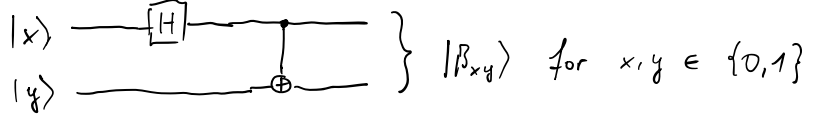
\includegraphics[scale=0.5]{chapters/res/circuit-bell-states.png}
    \caption{Quantum circuit to create Bell states}
\end{figure}


\subsection{Quantum teleportation}

Scenario: two (experimental physicists) Alice and Bob, are far away from each other

\begin{figure}[H]
    \centering
    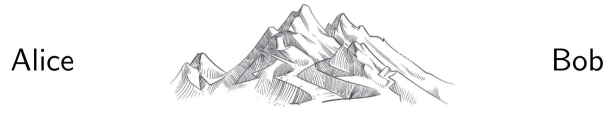
\includegraphics[scale=0.5]{chapters/res/alice-bob-mountains.png}
\end{figure}

When visiting each other a long time ago, they generated the EPR pair $\ket{\beta_{00}}$ each keeping on qubit of the pair.
Alice's task is to send another (unkown) qubit $\statepsi$ to Bob.
Note: Measurement is not an option.

\begin{figure}[H]
    \centering
    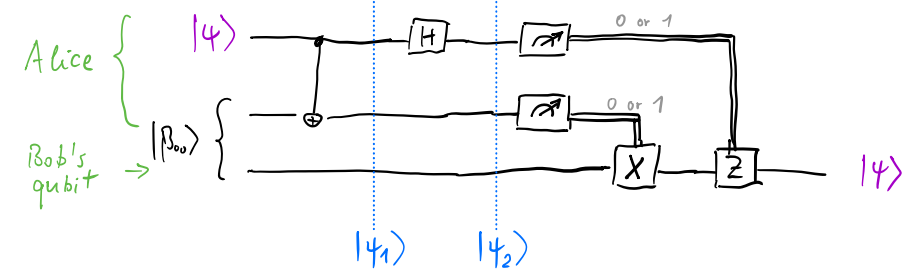
\includegraphics[scale=0.42]{chapters/res/circuit-teleporting-psi.png}
    \caption{Quantum circuit for teleporting $\statepsi$}
\end{figure}

Input:

\begin{equation*}
    \statepsi \ket{\beta_{00}} = (\alpha \ket{0} + \beta \ket{1}) \otimes \ket{\beta_{00}} 
        = \frac{1}{\sqrt{2}} \left[\alpha \ket{0} (\ket{00} + \ket{11}) + \beta \underbrace{\ket{1} (\ket{00} + \ket{11}}_{\text{CNOT}})\right]
\end{equation*}

after CNOT:
\begin{equation*}
    \ket{\psi_1} = \frac{1}{\sqrt{2}} 
        \left[\alpha \ket{0} (\ket{00} + \ket{11}) + \beta \ket{1} (\ket{{\color{red}1}0} + \ket{{\color{red}0}1})\right]
\end{equation*}

after Hadamard:
\begin{align*}
    \ket{\psi_2} &= \frac{1}{2} 
        [\alpha (\ket{0} + \ket{1})  \cdot
            (\ket{00} + \ket{11})]
        + \beta (\ket{0} - \ket{1}) \cdot 
            ((\ket{10} + \ket{01})) \\
    %
    &= \frac{1}{2} (\alpha \ket{000} + \alpha \ket{011} \alpha \ket{100} + \alpha \ket{111})
        + \beta \ket{010} + \beta \ket{001} - \beta \ket{110} - \beta \ket{101}) \\
    %
    &= \frac{1}{2} (\alpha \ket{000} + \alpha \ket{011} + \alpha \ket{100} + \alpha \ket{111}) + 
        \beta \ket{010} + \beta \ket{001} - \beta \ket{110} - \beta \ket{101} \\
    %
    &= \frac{1}{2} (\ket{00} (\alpha \ket{0} + \beta \ket{1}) + \ket{01} (\alpha \ket{1} + \beta \ket{0}))
        + \ket{10} (\alpha \ket{0} - \beta \ket{1}) + \ket{11} (\alpha \ket{1} - \beta \ket{0}))
\end{align*}

Now Alice measures her qubits w.r.t computational basis, e.g. projective measurement with 

\begin{align*}
    P_1 &= \ket{00} \bra{00} \otimes I, \quad P_2 = \ket{01} \bra{10} \otimes I \\ 
    P_3 &= \ket{10} \bra{10} \otimes I, \quad P_2 = \ket{11} \bra{11} \otimes I \\ 
\end{align*}

If Alice measures $\ket{00}$, then $\ket{\psi_2}$ will collapse to 
\begin{equation*}
    \ket{00} (\alpha \ket{0} + \beta \ket{1}) = \ket{00} \underbrace{\statepsi}_{\text{Qubit at Bob's place}}
\end{equation*}

similarly:

\begin{align*}
    00 &\mapsto \alpha \ket{0} + \beta \ket{1} \\
    01 &\mapsto \alpha \ket{1} + \beta \ket{0} \\
    10 &\mapsto \alpha \ket{0} - \beta \ket{1} \\
    11 &\mapsto \alpha \ket{1} - \beta \ket{0} 
\end{align*}

Alice transmits her measurement result to Bob (classical information), Bob then applies
Pauli-X and / or Pauli-Z to recover $\statepsi$. Even though wavefunction collapse is 
instantaneous, no faster-than-light transfer possible due to required classical communication.

\subsection{EPR and the Bell inequality}
EPR: Einstein, Podolsky, Rosen
EPR paper: \textit{"Can quantum mechanical description of physical relatiy be considered complete?"} (1935) \\
%
The another argue that quantum mechanics is incomplete since it lacks certain "elements of reality" 
(property can be predicted with certainity).

Scenario: Alice and Bob are far from each other, but share the entangled two-qubit "spin-singlet" state
\begin{equation*}
    \ket{\beta_{11}} = \frac{1}{\sqrt{2}} (\ket{01} - \ket{10})
\end{equation*}

Alice and Bob measure the observable $\vec{v} \circ  \vec{\sigma} = v_1 X + v_2 Y + v_3 Z$ 
(with $v \in \mathbb{R}^3, \norm{\vec{v}} = 1$) on their respective qubit.
(Recall $\vec{v} \circ \vec{\sigma}$ is Hermitian and unitary, and has eigenvalues $\pm 1$)

Alice performs her measurement immediately before Bob.
Example:
\begin{itemize}
    \item $\vec{v} = (0, 0, 1)^T$, observable $Z = 1 \cdot \ket{0} \bra{0} + (-1) \cdot \ket{1} \bra{1}$
        (standard measurement) \\
        if alice measures eigenvalue
        \begin{align*}
            1: &\quad \text{wavefunction collapses to } \ket{01} \\
            0: &\quad \text{wavefunction collapses to } \ket{10}
        \end{align*}
        $\leadsto$ Bob will always obtain the opposite measurement result.
    
    \item $\vec{v} = (1, 0, 0)^T$, observable: $X$, eigenstates 
    $\ket{\pm} = \frac{1}{\sqrt{2}}(\ket{0} + \ket{1})$, corresponding eigenvalues
    $\pm 1$ (measurement w.r.t $\{\ket{+}, \ket{-}\}$ basis) \\
    Can represent the wavefunction
    \begin{equation}
        \ket{\beta_{11}} = \frac{-1}{\sqrt{2}} (\ket{+-} - \ket{-+})
    \end{equation}
    namely:
        \begin{align*}
            \frac{-1}{\sqrt{2}} (\ket{+-} - \ket{-+}) 
                &= \frac{-1}{\sqrt{2}} ( \frac{1}{2} (\ket{0} + \ket{1})(\ket{0} - \ket{1})
                - \frac{1}{2}(\ket{0} - \ket{1})(\ket{0} + \ket{1})) \\
                &= ... = \frac{1}{\sqrt{2}} (\ket{01} - \ket{10}) = \ket{\beta_{11}}
        \end{align*}

    If Alice measures eigenvalue 1, wavefunction will tollapse to $\ket{+} \leadsto$ 
    Bob's qubit is in state $\ket{-}$, he will certainly measure eigenvalue $-1$.
    (Conversely if Alice measures -1)

    \item General observable $\vec{v} \circ \vec{\sigma}$, general unit vector 
    $\vec{v} \in \mathbb{R}^3$: \\
    Denote the orthogonal eigenstates of $\vec{v} \circ \vec{\sigma}$ by $\ket{a}$, $\ket{b}$,
    then there exist complex numbers $\alpha, \beta, \gamma, \delta \in \mathbb{C}$ such that

    \begin{align*}
        \ket{0} &= \alpha \ket{a} + \beta \ket{b} \\
        \ket{1} &= \gamma \ket{a} + \delta \ket{b}
    \end{align*}

    Inserted into $\ket{\beta_{11}}$ (see also Exercise 8.1 (a)):

    \begin{equation*}
        \frac{1}{\sqrt{2}} (\ket{01} - \ket{10}) 
            = \underbrace{(\alpha \delta - \beta \gamma)}_{
                    det(U) \text{ with } U = \begin{pmatrix*} 
                        \alpha & \beta \\ \gamma & \delta 
                    \end{pmatrix*}
                } \frac{1}{\sqrt{2}} (\ket{ab} - \ket{ba})
    \end{equation*}

    $U$ is base change matrix between orthonormal $\{ \ket{0}, \ket{1} \}$ and  
    $\{ \ket{0a}, \ket{b} \}$ basis $\leadsto U$ unitary $\leadsto \abs{det(U)} = 1$ (Exercise 1.2 (e)).

    Can represent $det(U) = e^{i \vartheta}, \vartheta \in \mathbb{R}$. \\
    In summary: 
    \begin{equation*}
        \frac{1}{\sqrt{2}} (\ket{01} - \ket{10}) 
            = e^{i \vartheta} \frac{1}{\sqrt{2}}(\ket{ab} - \ket{ba})
    \end{equation*}

    $\leadsto$ as before: Bob will obtain opposite measurement result as Alice.
    Therefore Alice can predict Bob's measurement result. \\
    However, there is no possibility that Alice could influence Bob's measurement result 
    (after performing her measurement) since they are far apart (speed of light too slow).
\end{itemize}

EPR argument: "Property" $\vec{v} \circ \vec{\sigma}$ of a qubit is an "element of reality".
However, quantum mechanics does not a priori specify this property for all possible $\vec{v}$ 
(but only probabilities), and is thus an incomplete description of reality. \\
Instead, "Hidden variable theory": There must be additional variables "hidden" in a qubit which
determine Bob's measurement of $\vec{v} \circ \vec{\sigma}$ for all possible $\vec{v} \in \mathbb{R}^3$. \\

Bell's inequality: Experimental test which can invalidate local hidden variable theories
(Bell 1964). \\

\underline{Local}: no faster-than-light communication possible 
(otherwise one could send information backwards in time according to special relativity). \\ 

Experimental schematic:  Many repetitions (to collect statistics) of the following setup:

\begin{figure}[H]
    \centering
    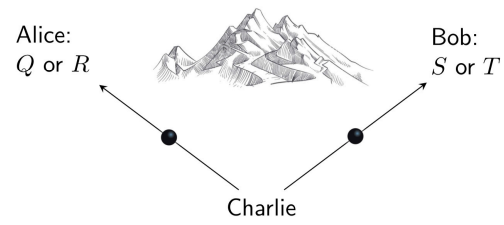
\includegraphics[scale=0.5]{chapters/res/alice-bob-charlie-mountain.png}
    \caption{Charlie prepares two particles, sends one to Alice and one to Bob.}
\end{figure}

By convention binary property values: $Q, R, S, T \in \{\pm 1 \}$. 
Alice decides randomly whether to measure property $Q$ or $R$ and Bob decides randomly to measure 
property $S$ or $T$. \\
Alice and Bob perform their measurement (almost) simultaneously, such that no information about their
result can be transmitted in between. \\ 
After completing this protocol, Alice and Bob need to analyse their measurement data. \\
Consider the quantity:
\begin{equation}
    QS + RS + RT - QT = \underbrace{(Q + R)}_{\pm 2 \text{ or } 0} S + \underbrace{(R - Q)}_{0 \text{ or } \pm 2} T
        = \pm 2
\end{equation}

Denote by $p(q, r, s, t)$ the probability that the system before the measurements is in state 
$Q = q, R = r, S = s, T = t$, then

\begin{align}
    \mathbb{E}[QS + RS + RT - QT] 
        &= \sum_{q, r, s, t \in \{\pm 1 \}} p(\underbrace{qs + rs + rt - qt}_{\pm 2}) \\ 
        %
        &\leq \sum_{q, r, s, t \in \{\pm 1 \}} p(q, r, s, t) \cdot 2 = 2 
\end{align}

By linearity of $\mathbb{E}$, arrive at the following \underline{Bell inequality}:

\begin{equation}
    \mathbb{E}[QS] + \mathbb{E}[RS] + \mathbb{E}[RT] - \mathbb{E}[QT]
        \leq 2
\end{equation}

Each term can be experimentally evaluated, e.g. for $\mathbb{E}[QS]$: \\
Alice and Bob average over cases where Alice measured $Q$ and Bob measured $S$. \\

Compare with "quantum" realization of the experiment: 
Charlie prepares two-qubit singlet state $\statepsi = \frac{1}{\sqrt{2}} (\ket{01} - \ket{10})$
and sends the first qubit to Alice and the second to Bob.
Observables
\begin{align*}
    Q &= \underbrace{Z_1}_{\text{acts on first qubit}}, 
        &&S = \frac{-Z_2 - X_2}{\sqrt{2}} \\
    %
    R &= X_1, &&T = \frac{Z_2 - X_2}{\sqrt{2}}
\end{align*}

Measurement averages (c.f. Exericse 8.1):
\begin{align*}
    \left\langle  QS \right\rangle &= \braketmatrix{\psi}{Q \otimes S}{\psi} = \frac{1}{\sqrt{2}} \\
    \left\langle  RS \right\rangle &= \frac{1}{\sqrt{2}} \\
    \left\langle  RT \right\rangle &= \frac{1}{\sqrt{2}} \\
    \left\langle  QS \right\rangle &= -\frac{1}{\sqrt{2}} 
\end{align*}

\begin{equation*}
    \leadsto  
        \left\langle  QS \right\rangle + 
        \left\langle  RS \right\rangle + 
        \left\langle  RT \right\rangle - 
        \left\langle  QT \right\rangle = 2 \sqrt{2} {\color{red} \nleq 2} \text{ (Violates Bell's inequality!)}
\end{equation*}

Actual labratory experiments (using photons) agree with predictions by quantum mechanics, 
thus not all (implicit) assumptions leading to Bell's inequality can be satisfied: \\

\begin{itemize}
    \item "realism": Physical properties $Q, R, S, T$ have definite values independent of observation
    (measurement).
    \item locality: Alice performing her measurement cannot influence Bob's measurement and vice versa
\end{itemize}

$\leadsto$  Nature is not "\textit{locally realistic}". 
(Most common viewpoint: Realism does not hold)

Practical lesson: Use entanglement as a resource.
\section{Quantum Search Algorithnms}
Classical search algorithm through $N$ unordered elements $\mathcal{O}(N)$. \\
Quantum Grover's algorithm: $\mathcal{O}(\sqrt{N})$ (given certain predictions).

\subsection{Quantum Oracles}
Search space of $N = 2^n$ elements, labelled $0, 1, ..., N - 1$.
Assume there are $M$ solutions (with $1 \leq M \leq N$). \\
Define corresponding indictor function $f : \{0, ..., N - 1\} \mapsto \{0, 1\}$
by 
\begin{equation}
    f(x) = \begin{cases}
        0, \quad \text{if element $x$ is not a solution} \\
        1, \quad \text{if element $x$ is a solution}
    \end{cases}
\end{equation}

Quantum version of $f$?
$\leadsto$ Quantum "oracle" $U_f$ defined for computational basis states as

\begin{figure}[H]
    \centering
    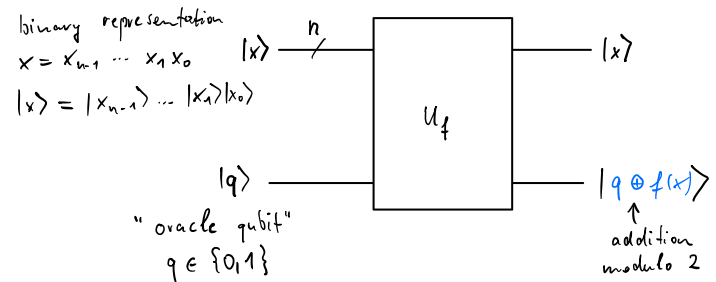
\includegraphics[scale=0.5]{chapters/res/quantum-circuit-oracle.png}
\end{figure}

Note: $U_f$ maps basis states to basis states and satisfies 
\begin{equation}
U_f^2 = I \quad (\text{since } q \oplus f(x) \oplus f(x) = q)
\end{equation}

Thus $U_f$ permutes basis states and is in particular unitary.

Initialize oracle qubit in superposition $\ket{-} = \frac{1}{\sqrt{2}}(\ket{0} - \ket{1})$, 
then 

\begin{equation}
    \ket{x} \otimes \frac{\ket{0} - \ket{1}}{\sqrt{2}}
    \stackrel{U_f}{\mapsto}
    \begin{cases}
        \ket{x} \otimes \frac{\ket{0} - \ket{1}}{\sqrt{2}} & \text{if } f(x) = 0\\
        \ket{x} \otimes \frac{\ket{1} - \ket{0}}{\sqrt{2}} = 
            - \ket{x} \otimes \frac{\ket{0} - \ket{1}}{\sqrt{2}} & \text{if } f(x) = 1
    \end{cases}
\end{equation}

In summary: 
\begin{equation}
    \ket{x} \otimes \frac{\ket{0} - \ket{1}}{\sqrt{2}}
    \stackrel{U_f}{\mapsto}
    \underbrace{{\color{blue}-1^{f(x)}}}_{\text{only this part relevant for the following}}
        \ket{x} \otimes \underbrace{\frac{\ket{0} - \ket{1}}{\sqrt{2}}}_{\text{Oracle qubit unchanged}}
\end{equation}

$\leadsto$ Effective action of oracle

\begin{figure}[H]
    \centering
    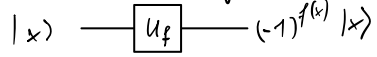
\includegraphics[scale=0.5]{chapters/res/effective-action-oracle.png}
    \caption{Oracle "marks" solution by a phase flip.}
\end{figure}


How could one construct such an oracle without knowing solution already? \\
Example: Factorization of a large integer $m \in \mathbb{N}$:
Finding prime factor of $m$ is "difficult" on a classical computer (no known algorithm with
polynomial runtime in the bit length of $m$). \\
But testing whether a given $x \in \mathbb{N}$ divides $m$ is simple.

Can perform arithmeti operations for trial divisions on a digital quantum computer as well
$\leadsto$ Oracle which recognizes a solution $x$.

\subsection{Grover's Algorithm}
Search space with $N = 2^n$ elements, $M$ solutions. 

\begin{figure}[H]
    \centering
    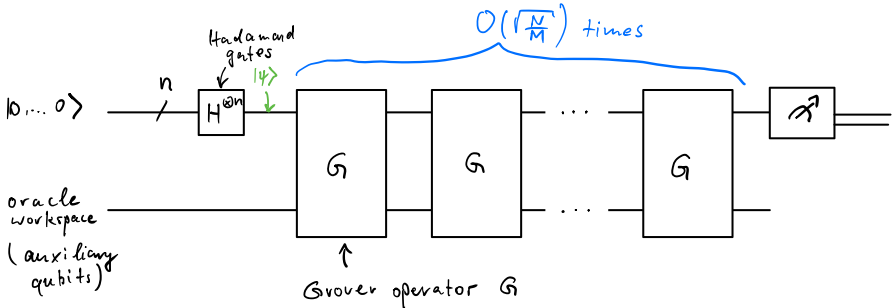
\includegraphics[scale=0.4]{chapters/res/groovers-algorithm.png}
\end{figure}

Initial Hadamard transform: \\

\begin{figure}[H]
    \centering
    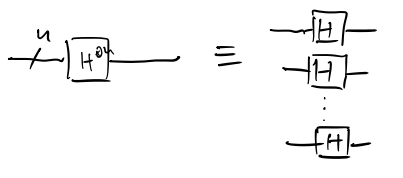
\includegraphics[scale=0.5]{chapters/res/initial-hadamard-transform.png}
\end{figure}
Note: For $x \in \{0, 1\}$:
\begin{equation}
    H \ket{x} = \frac{1}{\sqrt{2}} \sum_{z = 0}^1 (-1)^{z x} \ket{z} 
\end{equation}

Applied to several qubits:

\begin{align}
    H^{\otimes n} \ket{x_1, ..., x_n} 
        &= \underbrace{(H\ket{x_1})}_{\frac{1}{\sqrt{2}} \sum_{z_1 = 0}^1 (-1)^{x_1 z_1} \ket{z_1}}
            \otimes \cdots \otimes (H \ket{x_n}) \\ 
        % 
        &= \frac{1}{\sqrt{2^n}}  \sum_{z = 0}^{2^n - 1} (-1)^{x \cdot z} \underbrace{\ket{z}}_{\text{bit string}}
\end{align}

In particular: 
\begin{equation}
    H^{\otimes n} \ket{0, ..., 0} = \frac{1}{\sqrt{N}} \sum_{z = 0}^{N} \ket{z} =: {\color{green} \statepsi \text{ equal superposition state}}
\end{equation}

Definition of Grover operator G:

\begin{figure}[H]
    \centering
    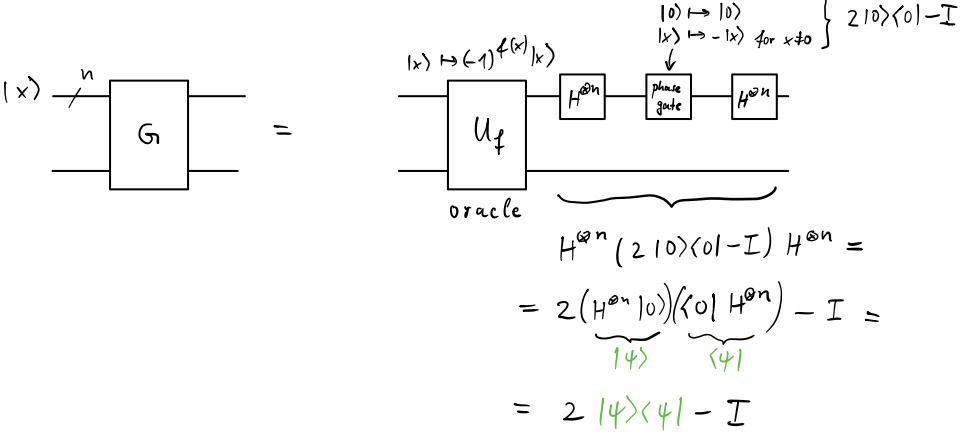
\includegraphics[scale=0.4]{chapters/res/grover-operation-circuit.png}
\end{figure}

In summary 
\begin{equation}
    G := (2 \statepsi \bra{\psi} - I) U_f
\end{equation}


\underline{Geometric interpretation:}

\begin{figure}[H]
    \centering
    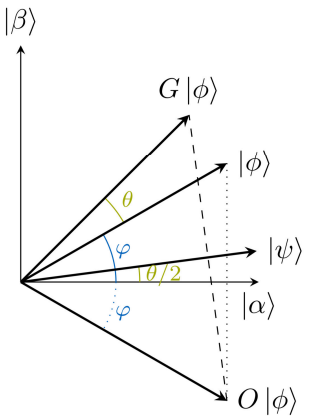
\includegraphics[scale=0.5]{chapters/res/grover-geometric-representation.png}
\end{figure}

Define 
\begin{equation}
    \ket{\alpha} := \frac{1}{\sqrt{N - M}} \sum_{x=0, f(x) = 0}^N \ket{x}
\end{equation}

\begin{equation}
    \ket{\beta} := \frac{1}{\sqrt{M}} \sum_{x=0, f(x) = 1}^N \ket{x}
\end{equation}


Angle $\vartheta$ defined by $\sin \frac{\vartheta}{2} = \sqrt{\frac{N}{M}}$
such that $\statepsi = \cos \frac{\vartheta}{2} \ket{\alpha} + \sin \frac{\vartheta}{2} \ket{\beta}$


Note: By definition $U_f \ket{a} = \alpha$, $U_f \ket{\beta} = -\ket{\beta}$ 
$\leadsto U_f$ is a reflection about $\ket{\alpha}$ within subspace spanned by $\ket{\alpha}$ and $\ket{\beta}$ \\

Likewise $2 \statepsi \bra{\psi} - I$ is a reflection about $\statepsi$:

\begin{figure}[H]
    \centering
    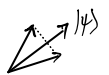
\includegraphics[scale=0.5]{chapters/res/psi-reflection-diagram.png}
\end{figure}

Since $\statepsi$ is part of subspace spanned by $\ket{\alpha}$ and $\ket{\beta}$, 
$G$ leaves subspace invariant! \\
Thus $G$ is a product of two reflections $\leadsto G$ is a rotation by angle 
$\vartheta$
\begin{align}
    \ket{\phi} &= \cos{\varphi} \ket{\alpha} + \cos{\varphi} \ket{\beta} \\
    \leadsto G \ket{\phi} &= \cos{(\varphi + \vartheta)} \ket{\alpha} + \cos{(\varphi + \vartheta)} \ket{\beta}
\end{align}
\section{The Density Operator}
So far: State vector $\statepsi$ describing a quantum state.
Convenient alternative formulation for quantum systems about which we 
only have partial information: \\
\underline{Density operator} (also called density matrix)

\subsection{Ensembles of quantum states}
Consider a quantum system which is in one of several states $\ket{\psi_i}$
with probability $p_i$: \underline{Ensemble} of quantum states
$\{p_i, \ket{\psi_i} \}$ \\
The \underline{density operator} $\rho$ of the ensemble $\{p_i, \ket{\psi_i} \}$
is defined as 

\begin{equation}
    \rho = \sum_i p_i \ket{\psi_i} \bra{\psi_i}
\end{equation}

Quantum mechanics in terms of the density operators:
\begin{itemize}
    \item Unitary operation: a unitary transformation $U$ maps each
    $\ket{\psi_i} \mapsto U \ket{\psi_i}$, and the ensemble to  $\{p_i, U \ket{\psi_i} \}$.
    Thus the density operator is transformed as 
    \begin{equation}
        \rho \stackrel{U}{\mapsto} \sum_i p_i U \ket{\psi_i} 
            \underbrace{\bra{\psi_i} U^\dag}_{(U\ket{\psi_i})^\dag} 
        = U \underbrace{(\sum_i p_i \ket{\psi_i} \bra{\psi_i})}_{\rho} U^\dag 
        = U \rho U^\dag
    \end{equation}

    \item Measurements: measurement operators $\{M_m\}$, if the system is in state
    $\ket{\psi_i}$, then the probability for result $m$, given $i$, is 
    \begin{equation}
        p(m|i) = \braketmatrix{\psi_i}{M_m^\dag M_m}{\psi_i} = 
            tr \left[ M_m^\dag M_m \ket{\psi_i} \bra{\psi_i} \right]
    \end{equation}
    Thus overall probability for result m is:
    \begin{align}
        p(m) &= \sum_i p(m|i) p_i = 
            \sum_i tr \left[ M_m^\dag M_m \ket{\psi_i} \bra{\psi_i} \right] p_i \\
            &= tr [ M_m^\dag M_m \underbrace{\sum_i p_i \ket{\psi_i} \bra{\psi_i}}_{\rho}] 
            = tr [M_m^\dag M_m \rho]
    \end{align}

    Density operator $\rho_m$ after obtaining measurement result $m$? \\
    State $i$ collapses to 
    \begin{equation}
    \ket{\psi_i} \mapsto \frac{M_m \ket{\psi_i}}{|| M_m \ket{\psi_i}||} =: \ket{\psi_i^m}
    \end{equation}
    Thus:
    
    \begin{align}
        \rho_m &= \sum_i p(i|m) \ket{\psi_i^m} \bra{\psi_i^m} 
            = \sum_i p(i|m) \frac{M_m \ket{\psi_i} \bra{\psi_i^m} M_m^\dag}
            {\underbrace{|| M_m \ket{\psi_i}||^2}_{p(m|i)}} \\
            &\stackrel{\text{Bayes Theorem}}{=} \sum_i p_i \frac{M_m \ket{\psi_i} \bra{\psi_i} M_m}{p(m)}
            = \frac{M_m \rho M_m^\dag}{tr[M_m^\dag M_m \rho]}
    \end{align}

    Note that $\rho_m$ is now expressed in terms of $\rho$ and the measurement
    operators, without explicit reference to the ensemble $\{p_i, \ket{\psi_i} \}$.
\end{itemize}

\subsection{General properties of the density operator}

Characterization of density operators: An operator $\rho$ is the
density matrix associated to some ensemble $\{p_i, \ket{\psi_i} \}$ if and only if:
\begin{enumerate}
    \item $tr[\rho] = 1$ (\textit{trace condition})
    \item $\rho$ is a positive operator (\textit{positivity condition})
\end{enumerate}
Remark: $\rho$ is called a \underline{positive operator} if it is Hermitian and all its
eigenvalues are non-negative, equivalent 
$\braketmatrix{\varphi}{\rho}{\varphi} \geq 0$ for all vectors $\ket{\varphi}$. 

Proof is in the official lecture notes on Moodle. \\

From now on, we define a density operator as positive operator $\rho$ with
$tr[\rho] = 1$. \\
Language regarding density operators: \\
\begin{enumerate}
    \item \underline{"Pure state"}: Quantum system in a state $\statepsi$, corresponding density 
operator $\rho = \statepsi \bra{\psi}$ such that 
\begin{equation}
    tr[\rho^2] = tr[\ket{\psi} \underbrace{\braket{\psi}{\psi}}_{1} \bra{\psi}] 
    = \braket{\psi}{\psi} = 1
\end{equation}

    \item \underline{"Mixed State"}: $\rho$ describing quantum setup cannot be written 
    as $\rho = \statepsi \bra{\psi}$; Intutition: Ensemble $\{p_i, \ket{\psi_i} \}$ of 
    $\rho$, all the probabilities are strictly smaller than 1. 
    Then $tr[\rho^2] = \sum_i p_i^2 < 1$.
\end{enumerate}

In general: Let $\rho$ be a density operator. Then  $tr[\rho^2] \leq 1$, 
and $tr[\rho^2] = 1$ if and only if $\rho$ describes a pure quantum state. \\
Proof: Denote the eigenvalues of $\rho$ by $\{\lambda_i \}$, then $- \leq \lambda_i \leq 1$
since $\rho$ is positive and $1 = tr[\rho] = \sum_i \lambda_i$.
Moreover, $tr[\rho^2] = \sum_i \lambda_i^2 \leq 1$, with "$=1$" precisely if one of the 
eigenvalues is 1 and the others are 0. \\


Ensemble representation is not unique! Example:
\begin{equation*}
    \rho = \frac{3}{4} \ket{0} \bra{0} + \frac{1}{4} \ket{1}\bra{1} 
    = \frac{1}{2} \ket{a} \bra{a} + \frac{1}{2} \ket{b}\bra{b} = 
\end{equation*}
with 
\begin{align*}
    \ket{a} &= \sqrt{\frac{3}{4}} \ket{0} + \sqrt{\frac{1}{4}} \ket{1} \\
    \ket{b} &= \sqrt{\frac{3}{4}} \ket{0} - \sqrt{\frac{1}{4}} \ket{1} \\
\end{align*}

(But note that $\ket{0}, \ket{1}$ are the (unique) eigenvectors of $\rho$, 
and $\braket{a}{b} \neq 0$.)


\end{document}